\subsection{Comparison with Previous Method}

At a high level, the objective of the measurement is to determine, from a third
point, if a {\reflector} blocks a blacklist IP. The blocking behavior that we
want to measure is \textit{inbound blocking} -- that is the incoming traffic
is blocked and as a result traffic does not reach the intended host. A
typical example is a network firewall, where it can stop certain network
packets from reaching hosts behind the firewall. Here I abstract the
{\reflector} as $Host_A$, blacklist IP as $Host_B$, and the problem is to
detect the connectivity between two hosts on the Internet.

\begin{figure}[t]
\centering
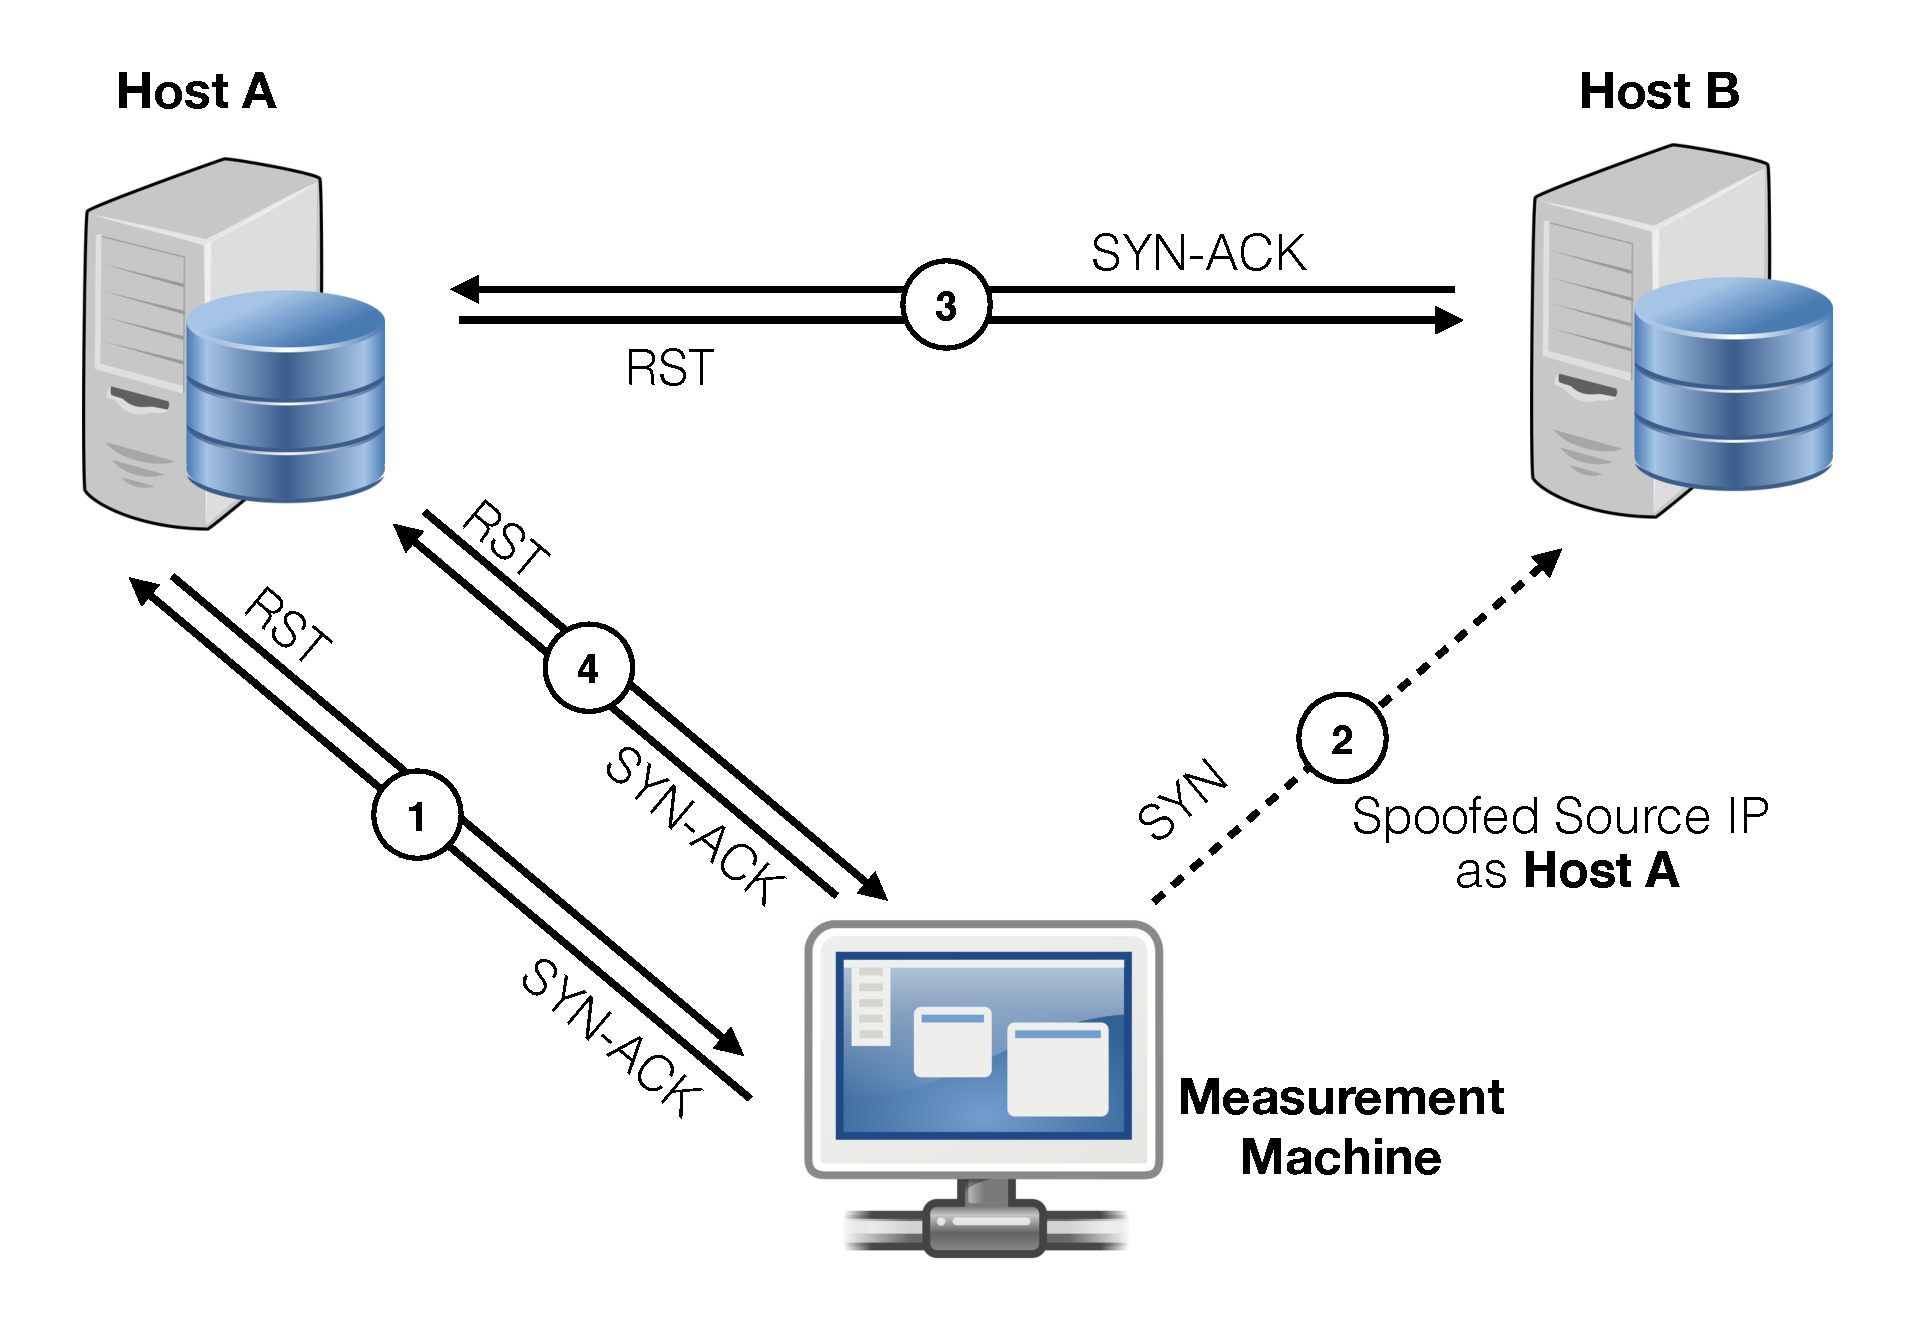
\includegraphics[width=0.8\columnwidth]{data_usage/images/croped_method_old.pdf}
\caption{Measurement method used in previous work.}
\label{fig:old_method}
\end{figure}

In previous works~\cite{pearce2017augur, ensafi2014detecting}, to measure
the connectivity between two hosts from a third party, they send spoofed packets
to impersonate one of the hosts. This methodology -- one I refer
to as the \textit{triangle measurement} takes advantage of the TCP 3-way
handshake protocol, as shown in Figure~\ref{fig:old_method}.

The measurement machine first sends a probe to the $Host_A$, in this case a TCP
SYN-ACK packet. $Host_A$ responds with a RST packet since it received a SYN-ACK
without the preceding SYN packet. Thus, the measurement machine gets the
first IP ID $IP\mhyphen ID_1$ from the RST packet (corresponds to Step 1 in
the figure). Next, the measurement machine sends a spoofed TCP SYN packet to
$Host_B$, with source IP address set to the IP address of $Host_A$ (Step 2).
$Host_B$ then sends a responding SYN-ACK packet to $Host_A$, which causes $Host_A$
to respond with a RST packet (Step 3), and increment its IP ID counter by 1.
Finally, the measurement machine probe $Host_A$ again and get the second IP ID
$IP\mhyphen ID_2$ (Step 4).

Now I can infer whether $Host_A$ is inbound blocking traffic from $Host_B$ by
observing the difference between $IP\mhyphen ID_1$ and $IP\mhyphen ID_2$.
Assuming there is no packet loss, and that $Host_A$ does not have any extra
traffic besides my measurement traffic, then
$IP\mhyphen ID_2 = IP\mhyphen ID_1 + 2$ implies there is no inbound blocking,
since it indicates that $Host_A$ received both packets in step 3 and step 4,
while $IP\mhyphen ID_2 = IP\mhyphen ID_1 + 1$ means there is blocking.

Previous work chose this ``triangle measurement'' because it ensures that in
step 3, the packets from $Host_B$ will go through the same routes as the
traffic originated from $Host_B$. So from $Host_A$'s perspective, it can not
identify that the traffic from $Host_B$ are spoofed. However, in this schema,
one hard requirement is that $Host_B$ needs to be active and responding to TCP
SYN probe. This is not an issue for censorship measurement, as $Host_B$ in this
case are popular sites (Google, Facebook, Twitter etc.) that guaranteed will
respond to SYN probe.

However, in this case, I need to measure whether $Host_A$ is blocking traffic
from a blacklist IP($Host_B$). But there is no guarantee that these IP
addresses are active and thus may not respond to the SYN probe. In fact, we
found that the percentage of responding IPs in a blacklist can be as low as less
than 20\%. This dramatically reduces the candidate IPs I can sample from a
blacklist to test, especially for small blacklists that only have a few hundred
IPs. Furthermore, there are many other additional constraints when shortlisting
IPs for measurement from a blacklist.
The requirement that blacklist IPs respond to SYN probe does not work for this
use case. 
%\textcolor{red}{Explain the choice for only inbound blocking}

In order to get around this limitation I adjust the measurement methodology.
In this new methodology, the measurement machine directly sends spoofed
packets to the target host, as shown in Figure~\ref{fig:new_method}. In
this case, the measurement machine first probes $Host_A$ to get the first IP ID
$IP\mhyphen ID_1$, then it sends a spoofed packet, with source IP set to
$Host_B$(Blacklist IP), directly to $Host_A$. Finally, it sends a second probe
to $Host_A$ and get the second IP ID $IP\mhyphen ID_2$. Now I can use the same
logic as before to infer whether $Host_A$ is inbound blocking $Host_B$. In this
approach, I do not require $Host_B$ to be actively responding SYN packets, any
IP address can be used here to conduct the test. The drawback is that the
spoofed packets now at times go through a different route versus the packets
originated from $Host_B$. Some network that implement spoofed packet
detection~\cite{ferguson2000rfc2827} could drop the spoofed packets, giving us
a false signal of inbound blocking. Therefore, when selecting hosts, I conduct
extensive tests to weed out hosts that have such detection logic in place. We
find that not a lot of target hosts have such detection logic. I will talk in
detail about host selection in the follow sections.

The disadvantage of this approach is that we cannot detect outbound 
blocking — wherein the spoofed packet reaches the reflectors but 
the responses are blocked when going out of the network
~\cite{pearce2017augur}. Based on our experience talking with several 
security companies, most customers deploy inbound blocking or 
bi-directional traffic blocking, so we do not think missing outbound 
blocking is a major concern.

\begin{figure}[t]
\centering
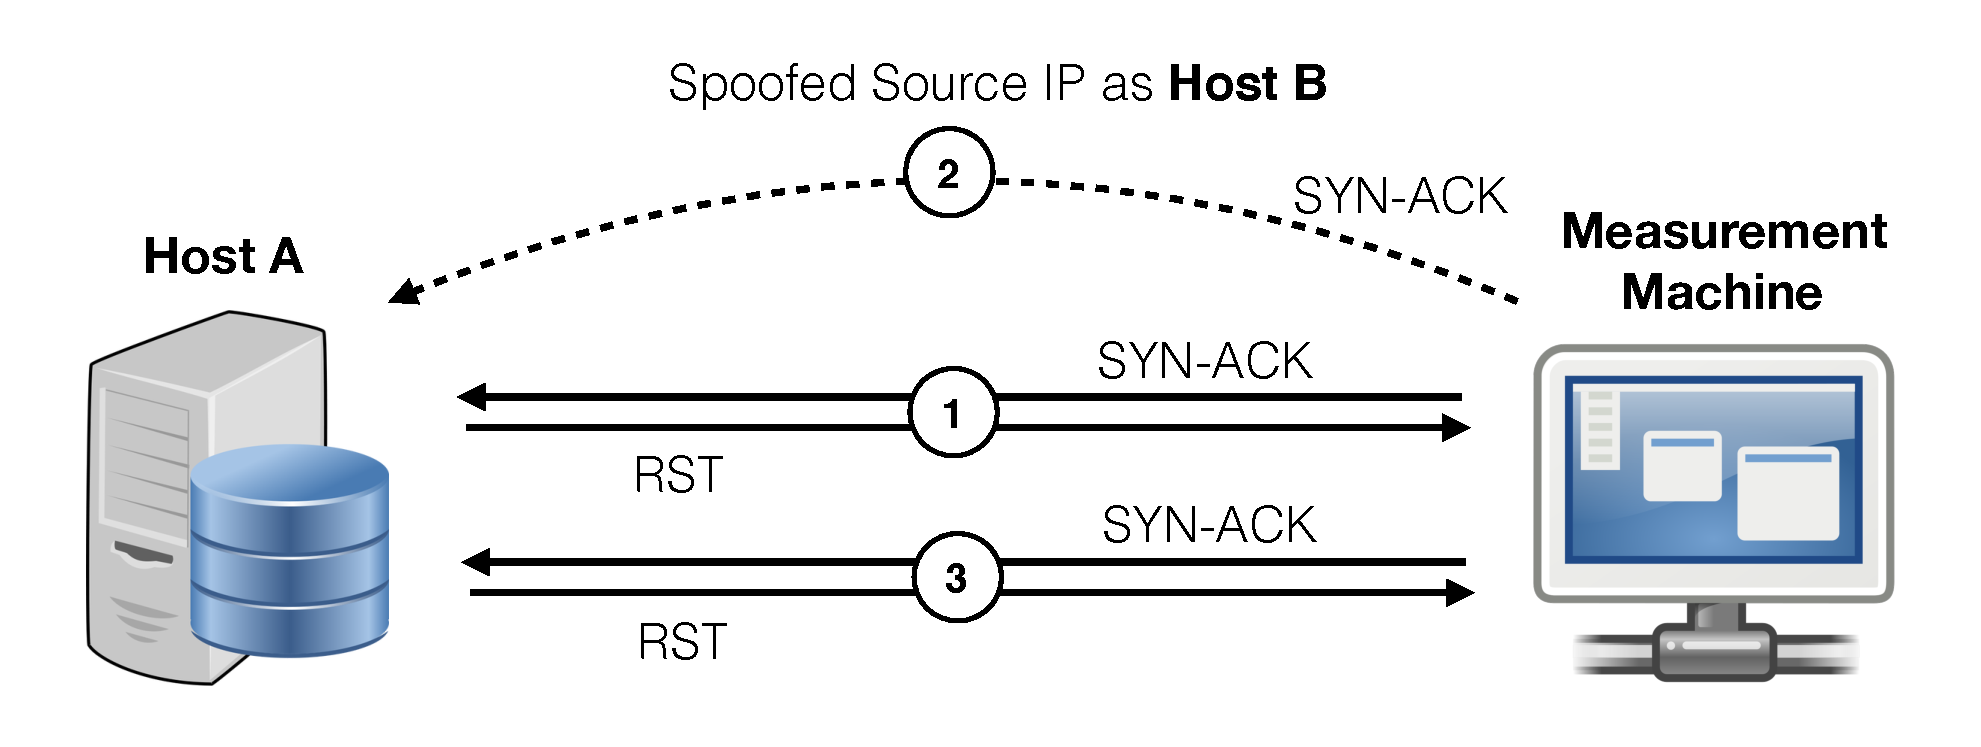
\includegraphics[width=0.8\columnwidth]{data_usage/images/croped_method_new.pdf}
\caption{Measurement method used in this work.}
\label{fig:new_method}
\end{figure}